% !TEX encoding = UTF-8 Unicode
\documentclass[11.2pt,twoside]{standalone}
\usepackage{tikz}
\usetikzlibrary{calc}
\usetikzlibrary{positioning}
\usepackage{tcolorbox}
\tcbuselibrary{skins}
\usepackage{fontspec,xunicode}
\setmainfont{Open Sans Condensed Light}
\definecolor{color1}{RGB}{245,172,216}
\definecolor{color2}{RGB}{235,92,178}
\def \regionUno{56}
\def \regionDos{4}
\def \regionTres{67}
\def \regionCuatro{17}
\def \regionCinco{34}
\def \regionSeis{31}
\def \regionSiete{12}
\def \regionOcho{55}

\thispagestyle{empty} 
\begin{document}

\begin{tikzpicture}
    \node[anchor=south west,inner sep=0] (image) at (0,0) {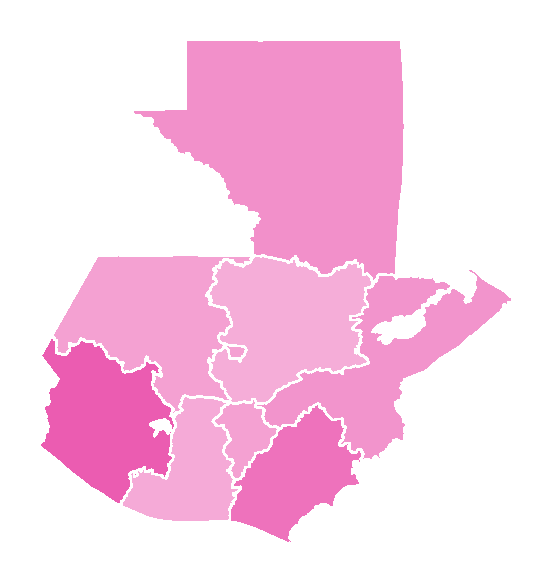
\includegraphics{mapa_sin_anotar}};
    \begin{scope}[x={(image.south east)}, y={(image.north west)}]

    % ###############REGION I############################## %
    \draw [black] (0.44,0.26) -- (0.44, 0.03);
    \filldraw [black] (0.44,0.26) circle (1.2pt);
    \draw [black] (0.44,0.03) -- (0.15,0.03	);
    \node[align=center,text width=3cm, color=black] at (0.08, 0.03) {Región I \\ \regionUno};
    
    %#############REGION II################################# %
	\filldraw [black] (0.52,0.44) circle (1.2pt);
    \draw [black] (0.52,0.44) -- (0.52, 0.59);
    \draw [black] (0.52,0.59) -- (0.9,0.59);
    \node[align=center,text width=3cm, color=black] at (0.98,0.59) {Región II \\  \regionDos};
    
    %#############REGION III################################# %
    \filldraw [black] (0.7,0.38) circle (1pt);
    \draw [black] (0.7,0.38) -- (0.97,0.38);
    \node[align=center,text width=3cm, color=black] at (1.05,0.38) {Región III \\  \regionTres};
    
    %#############REGION IV################################# %
    \filldraw [black] (0.53,0.18) circle (1pt);
    \draw [black] (0.53,0.18) -- (0.77,0.18);
    \node[align=center,text width=3cm, color=black] at (0.85,0.18) {Región IV \\  \regionCuatro};
    
    % ###############REGION V############################## %
    \filldraw [black] (0.34,0.19) circle (1pt);
    \draw [black] (0.34,0.19) -- (0,0.19);
%    \draw [black] (0.22,0.17) -- (0.22,0.24);
    \node[align=center,text width=3cm, color=black] at (-0.08,0.19) {Región V \\ \regionCinco};
    
    % ###############REGION VI############################## %
    \filldraw [black] (0.19,0.28) circle (1pt);
    \draw [black] (0.19,0.28) -- (0.19,0.6);
   \draw [black] (0.19,0.6) -- (0,0.6);
    \node[align=center,text width=3cm, color=black] at (-0.08,0.6) {Región VI \\ \regionSeis};
    
    % ###############REGION VII############################## %
    \filldraw [black] (0.28,0.45) circle (1pt);
    \draw [black] (0.28,0.45) -- (0.28,0.73);
    \draw [black] (0.28,0.73) -- (0,0.73);
    \node[align=center,text width=3cm, color=black] at (-0.08,0.73) {Región VII \\ \regionSiete };    
    
    %#############REGION VIII################################# %
    \filldraw [black] (0.54,0.75) circle (1pt);
    \draw [black] (0.54,0.75) -- (0.9,0.75);
    \node[align=center,text width=3cm, color=black] at (0.99,0.75) {Región VIII \\  \regionOcho };
    
    %################Barra#################################### %
    \shade[left color=color2,right color=color1] (0.3,0.97) rectangle (0.77,0.99);
    \node[align=right,text width=3cm, color=black] at (0.12,0.98) {Valor más grande};
    \node[align=left,text width=3cm, color=black] at (0.95,0.98) {Valor más pequeño};    
    
    \end{scope}
\end{tikzpicture}
\end{document}
